\documentclass[11pt]{article}
\usepackage[margin=1in]{geometry}
\usepackage{amsmath,amssymb}
\usepackage{graphicx}
\usepackage{caption}
\usepackage{hyperref}
\usepackage{enumitem}
\usepackage{booktabs}
\usepackage{array}

\newcommand{\indep}{\perp\!\!\!\perp}

\title{ECE 6257-GDL, Problem Set \#1\\
\large Solutions to Problems 1--8 and GDL-Bench Challenge Problem}
\author{Michael Incorvaia}
\date{}

\begin{document}
\maketitle
\tableofcontents
\newpage

\section{Problem 1: Data Generation in Low and High Dimensions}

We build an explicit generative model for $3\times 3$ binary images, recover
that same distribution from data with a learned scoring network, then examine
why the data-driven strategy collapses at $28\times 28$.

\subsection*{Part (a): An exact generative model for $3\times 3$ images}

Represent a $3\times 3$ black-and-white image as a binary vector
$x \in \{0,1\}^9$, where $1$ denotes ``black'' and $0$ denotes ``white,'' so
there are $2^9 = 512$ distinct images. We want
\[
  P(x) \;\propto\; \big(\text{number of black pixels in } x\big) \;=\; \sum_{i=1}^{9} x_i .
\]
Let $b(x) = \sum_{i=1}^{9} x_i$ be the black-pixel count. Each of the 9 pixels
is black in exactly half of the 512 images, so summing $b(x)$ over all images
normalizes the distribution,
\[
  Z \;=\; \sum_{x} b(x) \;=\; \sum_{i=1}^{9} \sum_{x} x_i \;=\; 9 \cdot 256 \;=\; 2304,
\]
giving the pmf
\[
  P(x) \;=\; \frac{b(x)}{2304}.
\]
The all-white image ($b(x)=0$) has probability exactly $0$, and the all-black
image ($b(x)=9$) is the single most likely image at $9/2304 \approx 0.0039$.

This is a Categorical distribution over the 512 images. We enumerate them as
categories $0,\dots,511$, assign each its probability $P(x)$, sample an index
from $\mathrm{Categorical}(P)$, and map it back to an image. Five samples drawn
this way are shown in Figure~\ref{fig:part_a}, and as expected, images with
many black pixels dominate.

\begin{figure}[h]
  \centering
  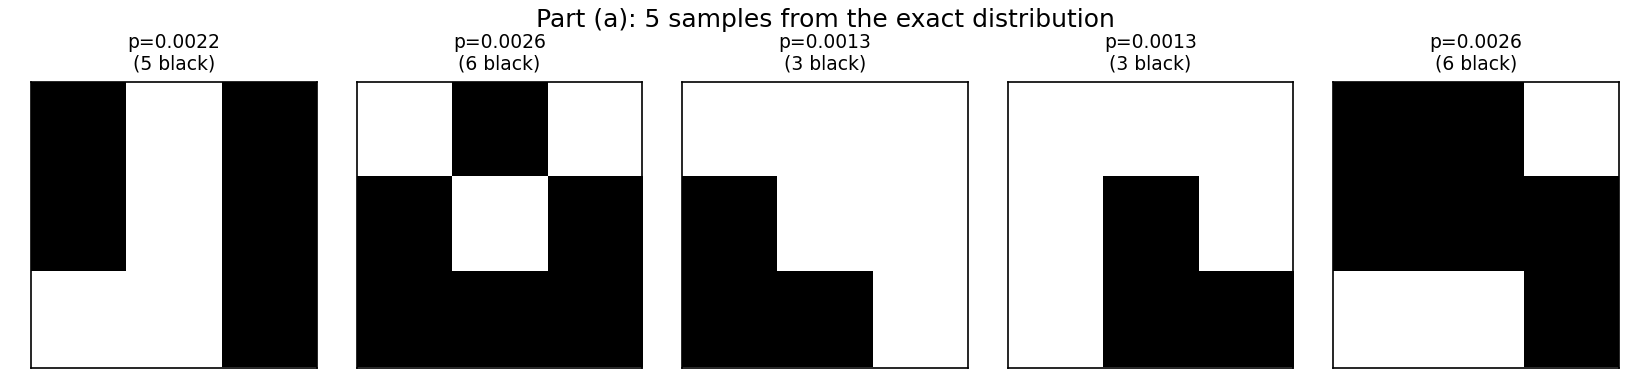
\includegraphics[width=\linewidth]{figures/part_a_samples.png}
  \caption{Five samples from the exact Categorical distribution
  $P(x) \propto (\text{number of black pixels})$. Titles show each sample's
  exact probability and black-pixel count.}
  \label{fig:part_a}
\end{figure}

\subsection*{Part (b): Learning the distribution from 200 labeled examples}

The generating rule is now treated as unknown. We are given 200 unique images
sampled from the part (a) distribution together with their true probabilities
$\{(x^{(j)}, P(x^{(j)}))\}_{j=1}^{200}$; 200 unique draws is possible because
511 of the 512 images have nonzero probability.

\paragraph{Model and target.} An MLP $f_\theta : \{0,1\}^9 \to \mathbb{R}$ takes
the flattened 9-pixel image and outputs a real-valued score. The raw
probabilities span more than an order of magnitude and are all tiny, so rather
than regressing them directly we regress the log-probability $y = \log P(x)$,
which is much better scaled for gradient-based training. The network has two
hidden layers of 64 ReLU units each, trained with Adam (MSE loss) until
convergence.

\paragraph{From scores back to a distribution.} After training, $f_\theta$ is
evaluated on all 512 possible images rather than only the 200 training images,
which we can afford only because the space is small enough to enumerate
exhaustively. Treating these scores as unnormalized log-probabilities, a
softmax converts them into a valid pmf,
\[
  \hat P(x) \;=\; \frac{\exp\big(f_\theta(x)\big)}{\displaystyle\sum_{x'} \exp\big(f_\theta(x')\big)},
\]
where the denominator sums over all 512 images. This is again a Categorical
distribution, now parameterized by the learned scores instead of the true
black-pixel count. On this run the MLP fits the 200 training points almost
exactly (training correlation $\approx 1.00$), and $\hat P(x)$ correlates with
the true $P(x)$ at $\approx 0.96$ across all 512 images, so the model has
essentially rediscovered ``more black pixels, higher probability'' from data
alone. Five samples from $\hat P(x)$ are shown in Figure~\ref{fig:part_b} and
again concentrate on images with several black pixels.

\begin{figure}[h]
  \centering
  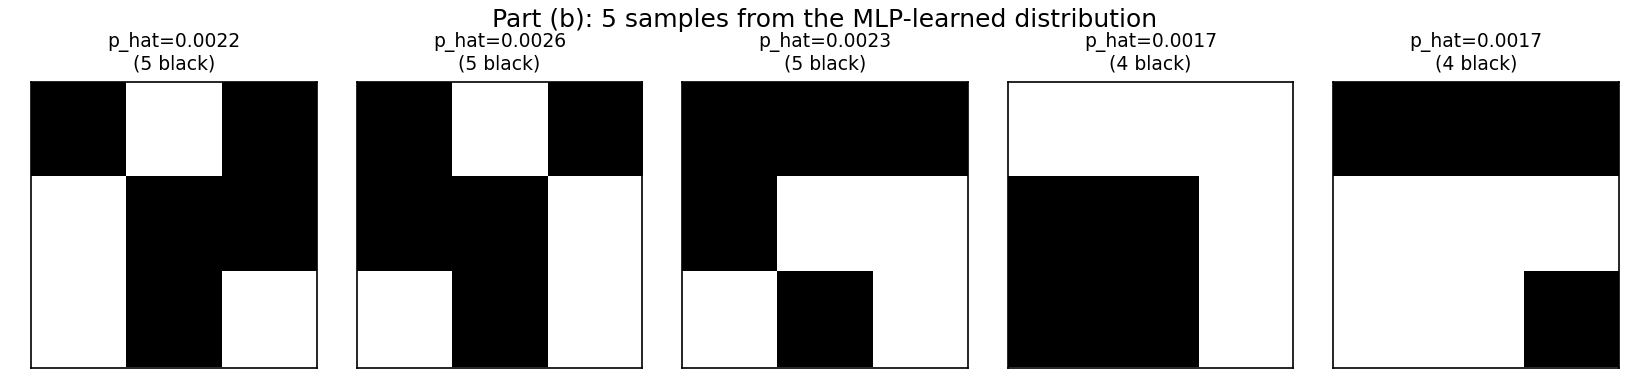
\includegraphics[width=\linewidth]{figures/part_b_samples.png}
  \caption{Five samples from the MLP-learned distribution $\hat P(x)$. Titles
  show the learned probability and true black-pixel count of each sample.}
  \label{fig:part_b}
\end{figure}

\begin{figure}[h]
  \centering
  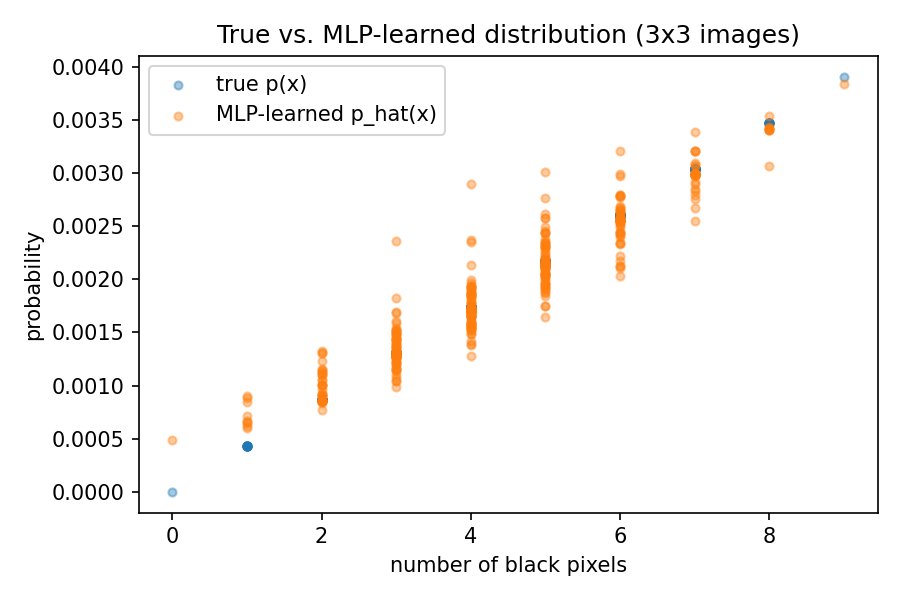
\includegraphics[width=0.7\linewidth]{figures/part_b_comparison.png}
  \caption{True probability $P(x)$ (blue) and MLP-learned probability
  $\hat P(x)$ (orange) for every one of the 512 possible images, plotted
  against black-pixel count. The learned distribution tracks the true linear
  trend closely, with some scatter because the network only ever saw 200 of
  the 512 images during training.}
  \label{fig:part_b_comparison}
\end{figure}

\subsection*{Part (c): Why this strategy fails at $28\times 28$}

The part (b) recipe, collect 200 (image, probability) pairs, fit an MLP,
evaluate it on all possible images, and re-normalize, breaks down as soon as
images grow from 9 pixels to 784. At least two independent reasons make it
infeasible.

\begin{enumerate}[label=\textbf{\arabic*.}, leftmargin=*]
\item \textbf{The image space can no longer be enumerated or normalized.}
Part (b) depends on evaluating the MLP on \emph{every} possible image and
summing the scores for the softmax normalizer $Z = \sum_{x} \exp(f_\theta(x))$,
which is affordable for $2^9 = 512$ images. At $28\times 28$ there are
$2^{784} \approx 10^{236}$ images, vastly more than the roughly $10^{80}$ atoms
in the observable universe, so enumerating that set, evaluating the network on
every element, or summing to get $Z$ is combinatorially impossible. This is
precisely the intractable-partition-function problem that motivates normalizing
flows, score-based and diffusion models, GANs, and autoregressive models, all
of which are built to sample from or evaluate high-dimensional distributions
without ever normalizing over the full space.

\item \textbf{200 examples cannot represent a 784-dimensional space.} In part
(b) the network saw 200 of 512 images, about 39\%, so it only had to
interpolate across a modestly under-sampled 9-dimensional input, where a small
MLP can still pick up a simple relationship between input and label. In 784
dimensions, 200 samples is an infinitesimal fraction of the space
($200/2^{784} \approx 0$) and, more importantly, is minuscule relative to the
input dimensionality itself. With far fewer examples than input features the
MLP can fit the 200 training points in ways that are completely arbitrary
everywhere else, the classic curse-of-dimensionality regime. The learned score
function is then essentially unconstrained over the vast majority of the space,
so scores far from the tiny training set are meaningless and the resulting
``distribution'' reflects nothing about the true data-generating process.

\item \textbf{(Bonus) High-dimensional structure is local and combinatorial.}
The $3\times 3$ label depends only on an additive statistic, pixel count, which
a small MLP recovers from relatively few points. Real image distributions
(digits, faces, natural scenes) have complex dependencies among pixels such as
edges, strokes, textures, and object structure, none of which can be inferred
from 200 scalar probability labels. There is simply not enough information in
the training set to identify a 784-dimensional density, however expressive the
network.
\end{enumerate}

In short, the part (b) strategy relies on exhaustively enumerating and
re-normalizing over the entire image space, and on 200 samples being
dense-enough coverage for an MLP to learn a meaningful score function. Both
assumptions hold at 9 pixels and both fail catastrophically at 784, which is
exactly why modern generative models are built around implicit sampling,
learned transformations of simple noise, autoregressive factorizations, and
score matching, none of which require enumerating or normalizing the full
high-dimensional space.

\paragraph{Reproducibility.} All numbers and figures above come from a single
self-contained Python script (\texttt{problem1.py}, using numpy, scikit-learn's
\texttt{MLPRegressor}, and matplotlib), included alongside this report.
\newpage
\section{Problem 2: Generative Modeling with an Independence Assumption (Binarized MNIST)}

We build a generative model for binarized MNIST digits under the assumption
that all 784 pixels are independent, derive the maximum likelihood estimate
(MLE) of its parameters, fit it to real data, generate new samples, and discuss
what the model can and cannot capture.

\subsection*{Model setup}

Each binarized MNIST image is a $28\times 28$ binary vector
$x = (x_1, \dots, x_D) \in \{0,1\}^D$ with $D = 784$, where a pixel is $1$ if
``on''/black and $0$ if ``off''/white. Under the independence assumption each
pixel $x_i$ is its own Bernoulli random variable with parameter
$\theta_i = P(x_i = 1)$, and the joint distribution factorizes as
\[
  p(x;\theta) \;=\; \prod_{i=1}^{D} \theta_i^{\,x_i} (1-\theta_i)^{\,1-x_i},
  \qquad \theta = (\theta_1, \dots, \theta_D).
\]
Every pixel location gets its own parameter, so the model does not assume
pixels share a value of $\theta$, only that they are statistically independent
once $\theta$ is fixed.

\subsection*{Likelihood of the dataset}

Given $N$ i.i.d.\ training images $\{x^{(1)}, \dots, x^{(N)}\}$, the likelihood
is a product of per-image likelihoods (independence across images), each itself
a product over the $D$ pixels (independence within an image),
\[
  L(\theta) \;=\; \prod_{n=1}^{N} p\big(x^{(n)}; \theta\big)
  \;=\; \prod_{n=1}^{N} \prod_{i=1}^{D}
  \theta_i^{\,x_i^{(n)}} (1-\theta_i)^{\,1-x_i^{(n)}}.
\]
Taking the log turns the double product into a double sum,
\[
  \ell(\theta) \;=\; \log L(\theta)
  \;=\; \sum_{n=1}^{N} \sum_{i=1}^{D}
  \Big[\, x_i^{(n)} \log \theta_i \;+\; \big(1-x_i^{(n)}\big) \log(1-\theta_i) \,\Big].
\]
Each $\theta_i$ appears in a separate additive term, so the log-likelihood
decomposes into $D$ independent one-dimensional problems, one per pixel,
\[
  \ell(\theta) \;=\; \sum_{i=1}^{D} \ell_i(\theta_i),
  \qquad
  \ell_i(\theta_i) \;=\; \sum_{n=1}^{N}
  \Big[\, x_i^{(n)} \log \theta_i \;+\; \big(1-x_i^{(n)}\big) \log(1-\theta_i) \,\Big].
\]

\subsection*{Maximum likelihood estimate}

For each pixel $i$, let $s_i = \sum_{n} x_i^{(n)}$ be the number of training
images in which pixel $i$ is on. Differentiating $\ell_i$ and setting it to
zero,
\[
  \frac{d\ell_i}{d\theta_i} \;=\; \frac{s_i}{\theta_i} \;-\; \frac{N-s_i}{1-\theta_i} \;=\; 0,
\]
and solving,
\[
  s_i(1-\theta_i) = (N-s_i)\theta_i
  \;\;\Longrightarrow\;\;
  s_i = N\theta_i
  \;\;\Longrightarrow\;\;
  \theta_i^{*} \;=\; \frac{s_i}{N} \;=\; \frac{1}{N}\sum_{n=1}^{N} x_i^{(n)}.
\]
The second derivative of $\ell_i$ is negative everywhere on $(0,1)$, confirming
this stationary point is a maximum. The MLE for each pixel is therefore the
empirical fraction of training images in which that pixel is on, so $\theta^{*}$
is exactly the pixel-wise average image,
\[
  \theta^{*} \;=\; \frac{1}{N}\sum_{n=1}^{N} x^{(n)}.
\]

\subsection*{Fitting the model to binarized MNIST}

We use the standard MNIST training set ($N = 50{,}000$ images, $784$ pixels
each), binarized with the deterministic threshold rule
$x_i = \mathbb{1}[\text{intensity}_i > 0.5]$. This is a deliberate choice, not
an oversight. The \texttt{binarized\_mnist} dataset commonly used for this
problem (e.g.\ via TFDS) ships a fixed \emph{stochastic} binarization following
Larochelle \& Murray (2011), where each pixel is sampled once as
Bernoulli(intensity), but both rules turn each pixel's grayscale intensity into
a black/white decision and are close enough here, so we use the simpler, fully
reproducible one. Computing $\theta^{*}$ element-wise over all 50{,}000 images
gives a 784-dimensional vector, reshaped to $28\times 28$ for visualization in
Figure~\ref{fig:theta_hat}. Its entries range from $0$ to about $0.56$, so no
single pixel is on in a majority of images once averaged across all ten digit
classes.

\begin{figure}[h]
  \centering
  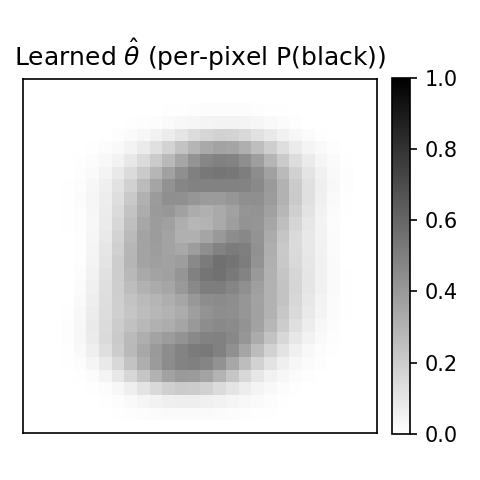
\includegraphics[width=0.45\linewidth]{figures/theta_hat.png}
  \caption{The learned parameter vector $\theta^{*}$, reshaped to
  $28\times 28$ and shown as a grayscale image (darker means higher
  probability of that pixel being black). This is exactly the pixel-wise
  average of every binarized training digit, and looks like a blurry,
  ghost-like superposition of all ten digit shapes.}
  \label{fig:theta_hat}
\end{figure}

\subsection*{Generating new images}

To sample a new image we draw every pixel independently,
$x_i \sim \mathrm{Bernoulli}(\theta_i^{*})$ for $i = 1, \dots, 784$, then
reshape to $28\times 28$. Ten samples are shown in Figure~\ref{fig:samples},
with ten real binarized digits in Figure~\ref{fig:real} for comparison.

\begin{figure}[h]
  \centering
  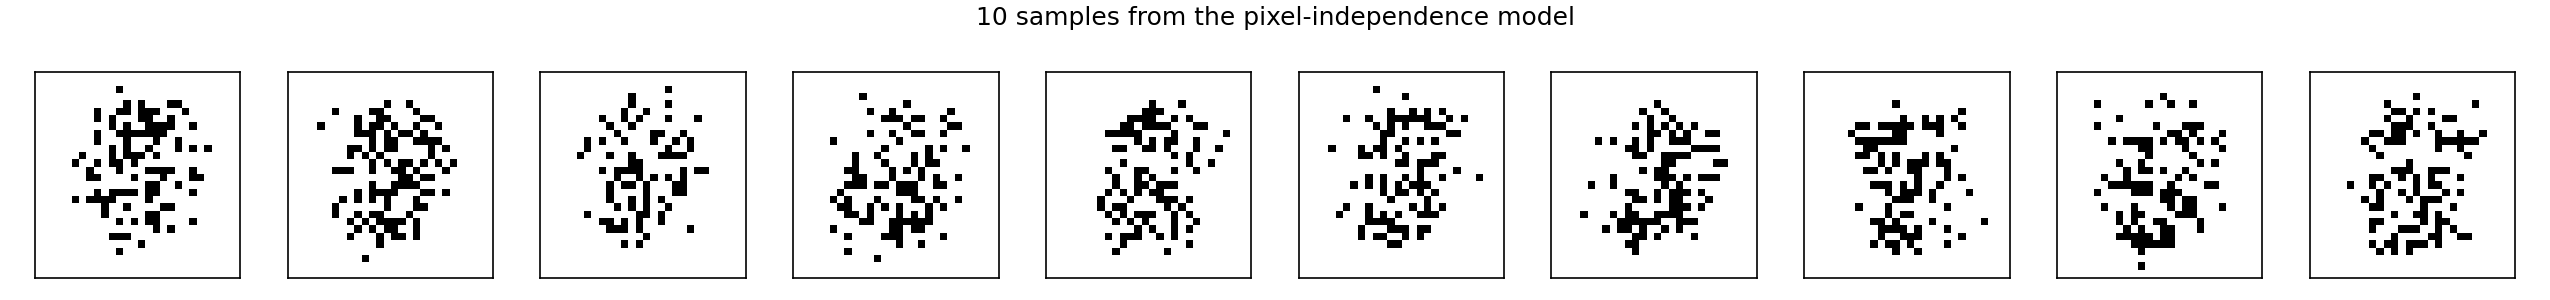
\includegraphics[width=\linewidth]{figures/independence_samples.png}
  \caption{Ten samples generated from the pixel-independence model,
  $x_i \sim \mathrm{Bernoulli}(\theta_i^{*})$ drawn independently per pixel.}
  \label{fig:samples}
\end{figure}

\begin{figure}[h]
  \centering
  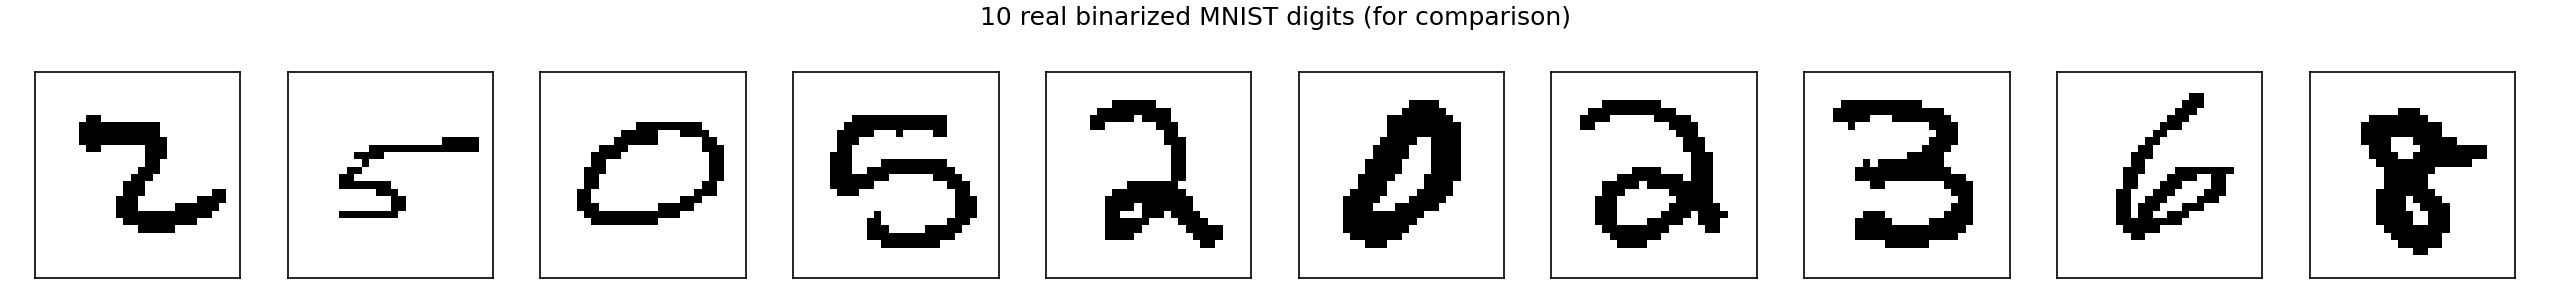
\includegraphics[width=\linewidth]{figures/real_examples.png}
  \caption{Ten real binarized MNIST training digits, shown for comparison.}
  \label{fig:real}
\end{figure}

\subsection*{Discussion: strengths and limitations of the independence assumption}

\paragraph{What the model captures.} The MLE $\theta^{*}$ exactly reproduces the
marginal per-pixel statistics of the training data, the probability that any
single pixel location is black averaged over the whole dataset. As
Figure~\ref{fig:theta_hat} shows, this recovers the coarse spatial envelope
where strokes tend to occur, with pixels almost always $0$ near the border,
since digits are centered and rarely touch the edges, and higher though still
well below $1$ in the central region where strokes from many digits overlap.
The model is also trivial to fit in closed form, one average per pixel, trivial
to sample from, and it is a valid, easy-to-normalize distribution over all
$2^{784}$ images, which the exhaustive-enumeration approach of Problem 1 could
never offer at this scale.

\paragraph{What the model fails to capture.} The samples in
Figure~\ref{fig:samples} do not look like digits at all; they look like
salt-and-pepper noise loosely concentrated in the center of the canvas. This
follows directly from the independence assumption. Because every pixel is
sampled on its own with no knowledge of any other pixel's value, the model
cannot represent the spatial correlations that make a digit recognizable, that
a stroke is a connected, continuous curve of adjacent black pixels rather than
a scattering of independently-lit dots, that particular combinations of strokes
form a loop (0, 6, 8, 9) or crossing lines (4, 7), and that the identity of the
whole digit constrains which pixels can plausibly be on \emph{together}. A pixel
being on at the top of a loop makes the matching pixel on the other side far
more likely to be on, not equally likely. None of this joint structure is
expressible by a product of independent marginals, since the model implicitly
assumes $P(x_i, x_j) = P(x_i)P(x_j)$ for every pair of pixels, which is badly
violated in real handwriting.

A second, related failure is that the model loses digit \emph{identity}.
Because $\theta^{*}$ is one fixed vector averaged across all ten classes, every
sample is drawn from the same distribution regardless of which digit it
``should'' be, so the model cannot even in principle produce a clean $0$ versus
a clean $7$; it has thrown away which pixels co-occur to form one class rather
than another. The same effect is visible in $\theta^{*}$ itself, which
resembles an overlapped blend of many digits rather than any one of them. The
independence assumption therefore captures first-order marginal statistics
correctly but discards all higher-order joint structure, and it is that
higher-order structure that makes an image look like a handwritten digit rather
than noise. Capturing it requires models that represent dependencies between
pixels, such as autoregressive models, latent-variable models like VAEs, Markov
random fields, or deep generative networks.

\paragraph{Reproducibility.} All numbers and figures come from a single
self-contained script (\texttt{problem2.py}), which loads the standard MNIST
training set, binarizes at a $0.5$ threshold, computes $\theta^{*}$ in closed
form, and draws samples with numpy.

\newpage
\section{Problem 3: Cats, Dogs, and DAGs}

\subsection*{The graph}

Let $S=$ Season, $P=$ Atmospheric Pressure, $A=$ Allergies, $R=$ Rain,
$G=$ Grass, $U=$ Umbrellas, $B=$ Dog Bark, $M=$ Cat Mood, $H=$ Cat Hide. The
DAG has edges
\[
  S\to A,\quad S\to R,\quad P\to R,\quad
  R\to G,\quad R\to U,\quad R\to B,\quad R\to M,\quad
  B\to H,\quad M\to H,
\]
shown in Figure~\ref{fig:dag}. Three structures do all the work. First, $S$ is
a fork (common cause) of $A$ and $R$. Second, $R$ is a fork of four downstream
effects $G,U,B,M$ and is itself a collider between two root causes $S$ and $P$.
Third, $B$ and $M$ are two causes colliding at $H$.

\begin{figure}[h]
  \centering
  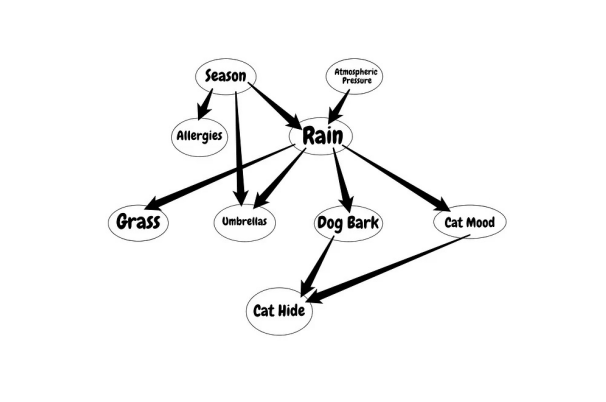
\includegraphics[width=0.75\linewidth]{figures/dag.png}
  \caption{The DAG under consideration.}
  \label{fig:dag}
\end{figure}

\subsection*{Rules used}

Two d-separation facts and one property of the factorization are all we need.

\begin{itemize}[leftmargin=*]
  \item \textbf{Chains ($X\to Z\to Y$) and forks ($X\leftarrow Z\to Y$)} are
  \emph{blocked} by conditioning on the middle node $Z$, giving
  $X \indep Y \mid Z$. Left unconditioned, the path is open and $X,Y$ are in
  general dependent.
  \item \textbf{Colliders ($X\to Z\leftarrow Y$)} behave oppositely. The path is
  \emph{blocked} by default, so $X \indep Y$ marginally, but becomes
  \emph{open} if $Z$ or any descendant of $Z$ is conditioned on, which in
  general makes $X$ and $Y$ dependent (``explaining away'').
\end{itemize}

A pair of nodes is conditionally independent given a set $Z$ exactly when
\emph{every} path between them is blocked given $Z$. We also use the
\textbf{local Markov property} implied by
$p(\text{all vars}) = \prod_i p(x_i \mid \text{parents}(x_i))$, namely that
every node is independent of its non-descendants given its parents.

\subsection*{Conditional independence relationships}

\paragraph{1. $A \indep R,P,G,U,B,M,H \mid S$.} Allergies' only parent is $S$,
and every other variable is a non-descendant of $A$, so by the local Markov
property conditioning on $S$ renders $A$ independent of everything else.
Equivalently, the only path out of $A$ is $A \leftarrow S \to R \to \cdots$, a
fork at $S$ that closes once $S$ is observed.

\paragraph{2. $S \indep P$ marginally, and $A \indep P$ marginally.} $S$ and $P$
are root nodes with no common ancestor, and their only connecting path is
$S \to R \leftarrow P$, a collider at $R$; an unconditioned collider blocks the
path, so they are marginally independent. The same mechanism gives a second
quick check, since $A$'s only connection to the rest of the graph runs through
$S$, making the sole path between $A$ and $P$ equal to
$A \leftarrow S \to R \leftarrow P$, still blocked at the same unconditioned
collider.

\paragraph{3. $S \indep P \mid R$ is \textbf{false}.} Conditioning on the
collider $R$, or on any descendant of $R$ such as $G$, $U$, $B$, $M$, or $H$,
\emph{opens} the path $S \to R \leftarrow P$. Observing that it rained, or that
the grass is wet, therefore makes $S$ and $P$ dependent even though they were
marginally independent. This is the classic explaining-away effect; if it
rained out of season, an unusual atmospheric-pressure event becomes more
likely, and vice versa.

\paragraph{4. $R \indep A \mid S$.} The only non-descendant of $R$ that is not
its parent is $A$, and the path $R \leftarrow S \to A$ is a fork at $S$, blocked
by conditioning on $S$. Once the season is known, whether it rains today says
nothing further about someone's allergies.

\paragraph{5. $G,U,B,M$ are mutually independent given $R$.} Take any two, say
$G$ and $U$; their only connecting path is $G \leftarrow R \to U$, a fork at $R$
blocked by conditioning on $R$. The same argument applies to every pair, so
\[
  G \indep U \mid R, \qquad G \indep B \mid R, \qquad G \indep M \mid R, \qquad
  U \indep B \mid R, \qquad U \indep M \mid R, \qquad B \indep M \mid R.
\]
Without conditioning on $R$ these are all dependent, since the fork through $R$
is open.

\paragraph{6. $B \indep M \mid R$, but $B \not\indep M \mid R, H$.} This is the
subtle version of point 5, worth stating separately because of $H$. $B$ and $M$
are independent given $R$, but they also collide at $H$
($B \to H \leftarrow M$), so conditioning on $H$ in addition to $R$ opens that
path and they become dependent again once the cat's hiding behavior is
observed. Concretely, if the dog did not bark ($B=0$) but the cat is hiding
anyway ($H=1$), a bad mood for some other reason ($M=1$) becomes more likely,
exactly the explaining away of point 3.

\paragraph{7. $H \indep S,P,R,G,U \mid B,M$.} Cat Hide's parents are $B$ and
$M$, and everything else is a non-descendant of $H$, so the local Markov
property gives independence from all of them given $\{B,M\}$. Intuitively, all
of $R$'s influence on hiding is assumed to be mediated through the dog's
barking and the cat's mood, so once those are known nothing further upstream
adds information.

\paragraph{8. Completing the local Markov property for $G,U,B,M$.} Points 5 and
6 state only \emph{pairwise} independencies among $G,U,B,M$ given $R$, but the
local Markov property is stronger, since each variable is independent of
\emph{every} non-descendant given its parents, not just of its three siblings.
Writing the full statement for each, and excluding for $B$ and $M$ their
descendant $H$, which is deliberately \emph{not} implied independent,
\[
  G \indep \{S,P,A,U,B,M,H\} \mid R, \qquad\quad
  U \indep \{S,P,A,G,B,M,H\} \mid R,
\]
\[
  B \indep \{S,P,A,G,U,M\} \mid R, \qquad\quad
  M \indep \{S,P,A,G,U,B\} \mid R.
\]
Each follows as in point 5, since $R$ is the only parent of $G,U,B,M$, so once
$R$ is fixed the only remaining paths out of each run back through $R$ (a fork,
blocked) or forward into the unconditioned collider at $H$ (blocked, for $B$ and
$M$). Nothing upstream of $R$, and none of the other three variables, carries
further information. This is what the pairwise statements leave implicit; it is
not just that $G,U,B,M$ stop depending on \emph{each other} once $R$ is known,
but that all four stop depending on everything upstream of $R$ as well.

\subsection*{Interpretation and evaluation}

\paragraph{Reasonable assumptions.}
\begin{itemize}[leftmargin=*]
  \item $S \indep P$ (point 2). Treating season and short-term pressure
  fluctuations as approximately independent root causes is a standard
  simplification in weather models, since day-to-day pressure systems are
  driven by processes not strongly locked to the calendar, at least compared to
  how strongly both drive rain.
  \item $G \indep U \mid R$, and similarly $U \indep B \mid R$ and
  $G \indep M \mid R$ (point 5). Wet grass, umbrellas, and a dog barking at the
  rain are all plausibly independent \emph{effects} of rain with no direct
  causal arrows between them; wet grass does not cause umbrellas, and vice
  versa. This is a reasonable use of a common cause to explain correlated
  observations without direct edges between every pair of effects.
  \item $H \indep R \mid B,M$ (point 7) is a reasonable mediation assumption
  \emph{if} the cat reacts only to the noise and mood consequences of rain
  rather than to rain itself, and it is a clean way to say rain affects the cat
  only indirectly.
\end{itemize}

\paragraph{Unrealistic assumptions.}
\begin{itemize}[leftmargin=*]
  \item $A \indep R \mid S$ (points 1 and 4) is questionable, since rain
  physically washes pollen out of the air and tends to \emph{reduce} allergy
  symptoms in the short term, independent of the seasonal pollen level. The
  graph forces all of rain's effect on allergies through season and misses this
  direct pathway, so a more realistic graph would include an edge $R \to A$.
  \item $B \indep M \mid R$ (points 5 and 6) assumes a barking dog has no direct
  effect on the cat's mood except through whatever made it bark. In reality a
  barking dog is quite likely to startle or agitate a nearby cat independent of
  rain, suggesting a missing edge $B \to M$, or a common unmodeled cause such as
  a loud noise outside.
  \item $H \indep R \mid B,M$ (point 7) is the shakiest of the mediation
  assumptions, since many cats hide directly in response to loud rain, thunder,
  or wind rather than only via a barking dog or a mood shift. If that direct
  pathway is meaningfully strong the independence would be violated in real
  data, and the graph should include an edge $R \to H$.
  \item $S \indep P$ (point 2) is fine as a first approximation but not
  perfectly realistic either, since pressure systems do have seasonal
  tendencies in many climates, so a small residual dependence is plausible even
  though the graph assumes none.
\end{itemize}

\paragraph{Summary.} The graph's independence claims are most trustworthy where
they encode separate downstream effects of a shared, already-identified cause,
with rain explaining grass, umbrellas, barking, and mood without direct links
between them. They are least trustworthy wherever a mediating variable is
assumed to fully screen off a more direct physical or behavioral pathway, as in
rain to allergies, dog bark to cat mood, and rain to cat hiding. The graph is a
useful simplification, but the mediation assumptions in particular should be
treated as modeling choices to check against data rather than as certainties.
\newpage
\section{Problem 4: Joint Distributions and Directed Cyclic Graphs}

\subsection*{Setup}

For a DAG, the factorization
\[
  p(x_1,\dots,x_n) \;=\; \prod_{i=1}^{n} p\big(x_i \mid \mathrm{pa}(x_i)\big)
\]
always defines a valid joint distribution. One can find a topological ordering
of the variables, parents before children, and marginalize them out one at a
time from the last variable backward; each conditional
$p(x_i \mid \mathrm{pa}(x_i))$ sums to $1$ over $x_i$ once all of $x_i$'s
descendants have been summed out, so the sum telescopes cleanly. The argument
relies entirely on such an ordering existing.

Now consider the directed \emph{cyclic} graph in Figure~\ref{fig:cyclic}, with
edges $A \to B$, $B \to C$, $C \to A$. Here $\mathrm{pa}(A) = \{C\}$,
$\mathrm{pa}(B) = \{A\}$, and $\mathrm{pa}(C) = \{B\}$, so the analogous
factorization would be
\[
  p(a,b,c) \;=\; p(a \mid c)\, p(b \mid a)\, p(c \mid b).
\]
Because the graph has a cycle $A \to B \to C \to A$ there is no topological
ordering, so the telescoping argument does not apply. We show by explicit
counterexample that this factorization can fail to be a valid joint
distribution, since the right-hand side need not sum to $1$.

\begin{figure}[h]
  \centering
  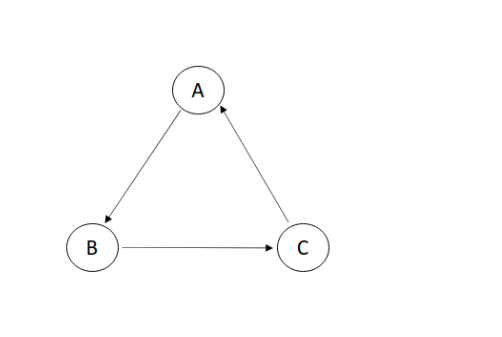
\includegraphics[width=0.5\linewidth]{figures/cyclic_dag.png}
  \caption{The directed cyclic graph under consideration, $A\to B\to C\to A$.}
  \label{fig:cyclic}
\end{figure}

\subsection*{Counterexample}

Let $A,B,C \in \{0,1\}$ and choose each conditional to be the (valid)
\emph{deterministic identity} map from parent to child,
\[
  p(a \mid c) = \mathbf{1}[a = c], \qquad
  p(b \mid a) = \mathbf{1}[b = a], \qquad
  p(c \mid b) = \mathbf{1}[c = b].
\]
Each is a perfectly valid conditional distribution, since for every fixed value
of the conditioning variable the two outcomes of the child are non-negative and
sum to $1$; for instance $p(A=0\mid C=0)=1$ and $p(A=1\mid C=0)=0$, and likewise
for $C=1$ and for the other two conditionals.

Multiplying according to the cyclic factorization gives
\[
  p(a,b,c) \;=\; \mathbf{1}[a=c]\,\mathbf{1}[b=a]\,\mathbf{1}[c=b]
  \;=\; \mathbf{1}[a=b=c],
\]
since the product of the three indicators is $1$ exactly when $a=c$, $b=a$, and
$c=b$ hold simultaneously, i.e.\ when $a=b=c$, and $0$ otherwise. Evaluating at
all $2^3 = 8$ binary assignments,

\begin{table}[h]
\centering
\begin{tabular}{ccc|c}
\toprule
$a$ & $b$ & $c$ & $p(a\mid c)\,p(b\mid a)\,p(c\mid b)$ \\
\midrule
0 & 0 & 0 & $1 \cdot 1 \cdot 1 = 1$ \\
0 & 0 & 1 & $0 \cdot 1 \cdot 0 = 0$ \\
0 & 1 & 0 & $1 \cdot 0 \cdot 0 = 0$ \\
0 & 1 & 1 & $0 \cdot 0 \cdot 1 = 0$ \\
1 & 0 & 0 & $0 \cdot 0 \cdot 1 = 0$ \\
1 & 0 & 1 & $1 \cdot 0 \cdot 0 = 0$ \\
1 & 1 & 0 & $0 \cdot 1 \cdot 0 = 0$ \\
1 & 1 & 1 & $1 \cdot 1 \cdot 1 = 1$ \\
\bottomrule
\end{tabular}
\end{table}

\noindent and summing the last column over all 8 rows,
\[
  \sum_{a\in\{0,1\}}\sum_{b\in\{0,1\}}\sum_{c\in\{0,1\}}
  p(a\mid c)\,p(b\mid a)\,p(c\mid b)
  \;=\; \underbrace{1}_{(0,0,0)} + \underbrace{1}_{(1,1,1)} + 0+0+0+0+0+0
  \;=\; 2 \;\neq\; 1.
\]
A valid joint pmf over $(A,B,C)$ must sum to exactly $1$, so this function is
\textbf{not} a valid joint distribution even though every individual factor is
itself a perfectly valid conditional distribution. This is the required
counterexample; naively applying the DAG factorization formula to a cyclic
graph does not in general produce a properly normalized joint distribution.

\subsection*{Why this happens}

The proof that the DAG factorization normalizes works by picking a topological
order $x_{\pi(1)}, \dots, x_{\pi(n)}$, every parent before its children, and
marginalizing from the last variable to the first. The step
\[
  \sum_{x_{\pi(n)}} p\big(x_{\pi(n)} \mid \mathrm{pa}(x_{\pi(n)})\big) = 1
\]
removes $x_{\pi(n)}$ for free, since its parents are all among the remaining
variables and the sum leaves the rest of the product untouched, and repeating
for $x_{\pi(n-1)}, \dots, x_{\pi(1)}$ eventually leaves
$\sum_{x_{\pi(1)}} p(x_{\pi(1)}) = 1$. Every step requires the variable being
summed out to not be a parent of any \emph{remaining} variable, which is exactly
what a topological order guarantees.

In the cyclic graph no such order exists, since $A$ is a parent of $B$ but also
a child of $C$, which is a child of $B$; whichever variable we sum out first is
simultaneously an ancestor of another variable still in the product, and the
cancellation breaks down. Our counterexample realizes this concretely, since
forcing $A=C$, $B=A$, and $C=B$ at once is an over-constrained, circular set of
requirements that happens to admit two consistent solutions, $a=b=c=0$ and
$a=b=c=1$, instead of the single degree of freedom a valid normalized chain
would have. That is why the total mass doubles rather than summing to $1$.

\newpage
\section{Problem 5: NADE and MADE on MNIST}

\subsection*{Setup}

We compare two neural autoregressive density estimators, NADE (Larochelle \&
Murray, 2011) and MADE (Germain et al., 2015), on binarized MNIST, using the
reference implementations from
\href{https://github.com/EugenHotaj/pytorch-generative}{EugenHotaj/pytorch-generative}.
Both factor the joint pixel distribution autoregressively,
\[
  p(x) = \prod_{i=1}^{784} p\big(x_i \mid x_{<i}\big),
\]
but parameterize the conditionals differently. NADE ties weights across a
single hidden layer via a cumulative-sum recurrence over a fixed pixel order,
while MADE masks the connections of an ordinary feedforward network so that
unit $i$'s output depends only on inputs before it in some (possibly random)
order.

For a controlled comparison we trained both for $30$ epochs with hidden
dimension $300$, batch size $512$, Adam with default hyperparameters, and
dynamically binarized MNIST, resampling each pixel as Bernoulli($x_i$) every
epoch so neither model memorizes a fixed binarization. With these settings both
have an \emph{identical} parameter count of $471{,}484$, since NADE's
$784 \times 300$ and $300\times784$ weight matrices are the same shape as MADE's
single-hidden-layer mapping $784 \to 300 \to 784$. The comparison is therefore
about how the two models use that capacity, not how much they have.

\paragraph{An implementation bug and its fix.} While training NADE the loss
plateaued almost immediately at $\approx 539$ nats/image, suspiciously close to
the chance level of $784\ln 2 \approx 543.4$ nats, the loss a model assigning
$p=\tfrac12$ to every pixel would achieve. The cause was a real bug in the
reference \texttt{reproduce()} function. NADE's \texttt{forward} already applies
a sigmoid internally and returns $\hat p$, a probability rather than a logit,
but the reference training loop feeds this into
\texttt{binary\_cross\_entropy\_with\_logits}, which silently applies a
\emph{second} sigmoid. Composing two sigmoids squashes the effective output into
a narrow band around $0.5$ and crushes the gradient, so the model can never
learn confident pixel probabilities. MADE has no such issue, since its final
masked linear layer has no trailing activation and genuinely does output
logits, making the reference loss correct for it. We replaced NADE's loss with
plain binary cross-entropy on probabilities and retrained from scratch, after
which the eval loss dropped from $\approx 539$ to $\approx 97$ nats within $7$
epochs and converged normally. All results below use the corrected NADE.

\paragraph{A note on training.} Long-running background training processes in
our execution environment did not reliably survive between tool invocations,
since the sandbox container could be recycled, so instead of one uninterrupted
30-epoch run we trained NADE in short checkpointed foreground chunks, saving
model and optimizer state after every epoch and resuming from the last
checkpoint. This is behaviorally identical to a single continuous run.

\subsection*{Part (a): NADE}

NADE was trained for the full $30$ epochs. Held-out loss decreased smoothly and
monotonically, from $97.5$ nats/image after epoch $7$ to a final eval loss of
$90.1$ nats/image (train loss $90.5$) at epoch $30$
(Figure~\ref{fig:losses}).\footnote{Because of the checkpointed training,
held-out loss for NADE was logged only at epochs $7, 14, 21, 28, 30$, so
``smoothly and monotonically'' describes the trend across those five
checkpoints rather than a continuous per-epoch curve.} Twenty samples drawn by
ancestral sampling in raster order, pixel by pixel, are shown in
Figure~\ref{fig:nade}.

\begin{figure}[h]
  \centering
  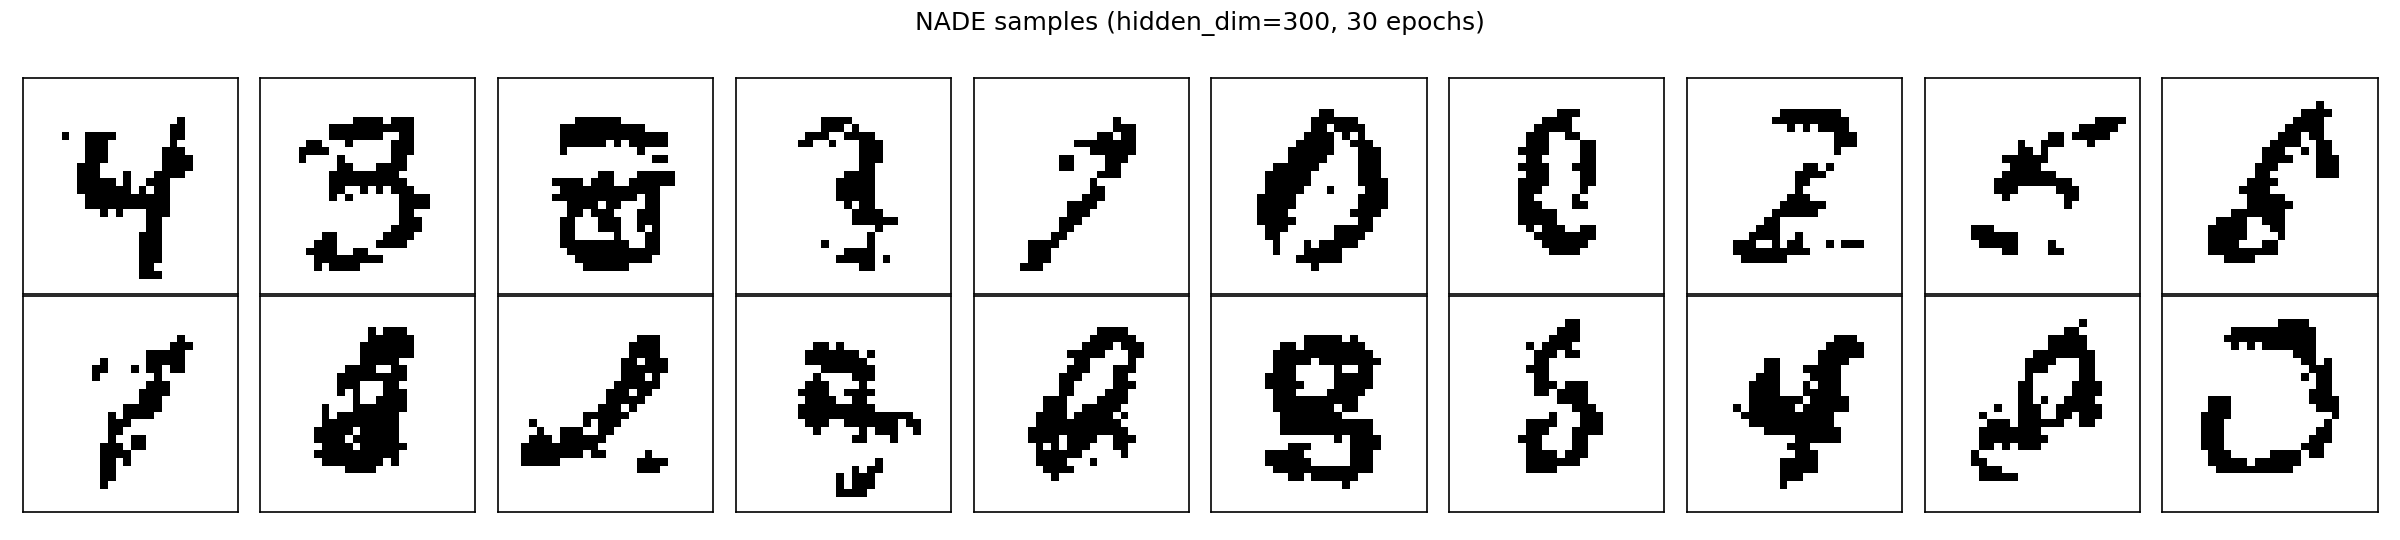
\includegraphics[width=\textwidth]{figures/nade_samples.png}
  \caption{20 samples from NADE (hidden\_dim$=300$, 30 epochs).}
  \label{fig:nade}
\end{figure}

The samples are clearly recognizable digits (4, 3, 7, 1, 0, 2, 8, 5, and
others) with mostly coherent, connected strokes, some smooth curvature, and
only mild speckle noise around the edges of a few characters, a strong result
for such a small single-hidden-layer model.

\subsection*{Part (b): MADE and comparison}

MADE was trained identically, same $30$ epochs, hidden dimension $300$
(\texttt{hidden\_dims=[300]}), a single mask ($n\_masks=1$), batch size $512$,
and Adam. Its held-out loss also decreased smoothly, from $211$ nats after
epoch $1$ to $100.5$ nats/image at epoch $30$ (train loss $104.7$); see
Figure~\ref{fig:losses}. Twenty samples are shown in Figure~\ref{fig:made}.

\begin{figure}[h]
  \centering
  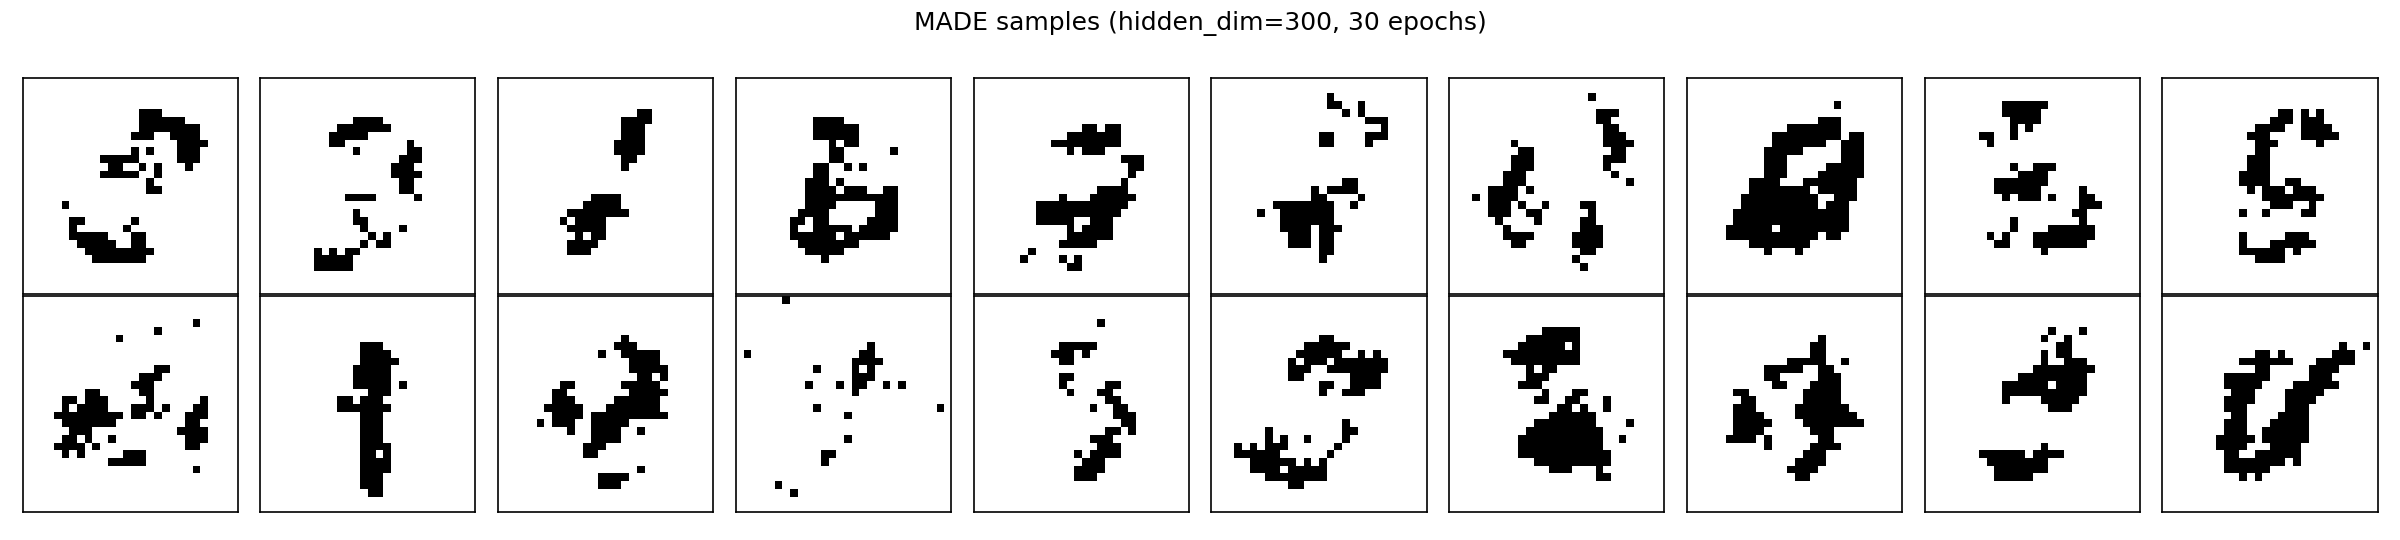
\includegraphics[width=\textwidth]{figures/made_samples.png}
  \caption{20 samples from MADE (hidden\_dims$=[300]$, $n\_masks=1$, 30 epochs).}
  \label{fig:made}
\end{figure}

\begin{figure}[h]
  \centering
  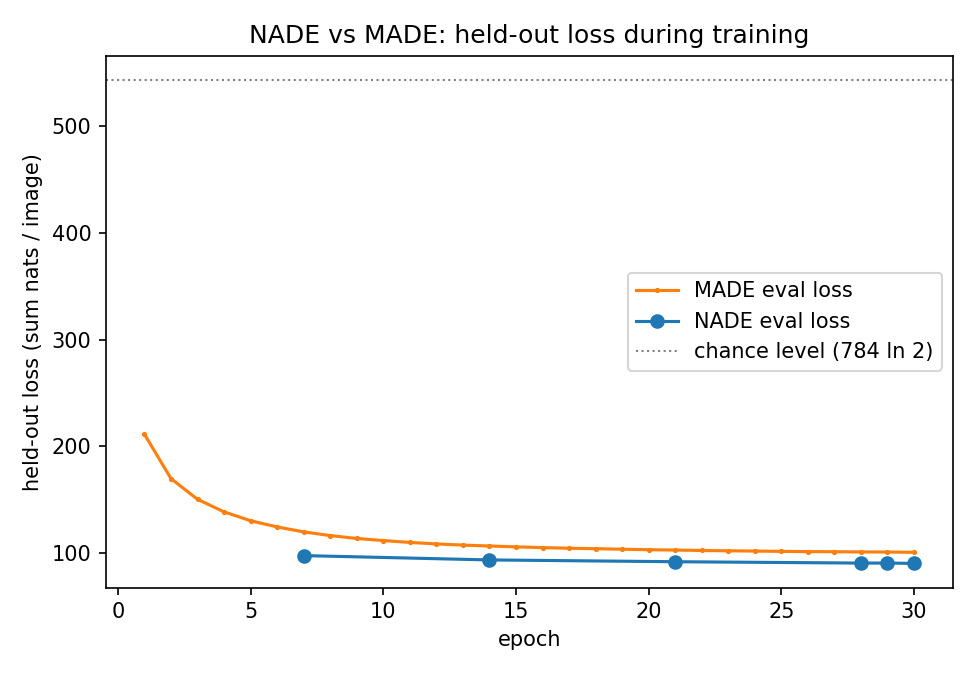
\includegraphics[width=0.75\textwidth]{figures/loss_comparison.png}
  \caption{Held-out loss during training for NADE and MADE.}
  \label{fig:losses}
\end{figure}

\paragraph{Which looks more plausible?} NADE's samples are unambiguously more
plausible MNIST digits. MADE's are visually much worse despite only a slightly
higher held-out loss, about $10$ nats/image, and consist mostly of disconnected
blobs and streaks with little recognizable digit structure, though a handful
such as a loopy ``0''-like shape hint at it.

Given identical parameter counts, three architectural properties explain the
gap between likelihood and sample quality.

\begin{itemize}
  \item \textbf{Pixel ordering.} NADE conditions in raster (row-major) order,
  which respects image structure, since the pixels immediately before pixel $i$
  are literally its neighbors above and to the left. MADE with a single random
  mask conditions on a \emph{random permutation} of the 784 pixels, and a random
  order has no relationship to spatial adjacency, so a pixel deep inside a
  digit may have to be predicted from a ``before'' set consisting mostly of
  pixels scattered elsewhere, with few of its true neighbors available yet.
  \item \textbf{Weight tying versus a shallow masked MLP.} NADE's hidden
  activation is built by an explicit recurrence,
  $a_i = a_{i-1} + x_{i-1} W_{:,i-1}$, so every conditional reuses the same
  accumulated hidden state and the same weight matrix column by column, a
  strong and useful inductive bias for a sequential, spatially structured
  signal. MADE with one hidden layer and one mask is architecturally just a
  masked single-hidden-layer MLP with no recurrence or weight sharing across
  autoregressive steps, so it must fit all 784 conditionals with comparatively
  unstructured, independent capacity.
  \item \textbf{Compounding sampling errors.} Both models are trained with
  teacher forcing, so the loss reflects one-step-ahead accuracy conditioned on
  \emph{true} previous pixels. During sampling they condition on their own
  previously \emph{generated} pixels, and errors compound over 784 sequential
  steps. MADE's random order and unshared weights give it a weaker spatial
  prior, so small early mistakes are more likely to cascade into globally
  incoherent images, whereas NADE's raster order and weight-tied recurrence make
  it more robust.
\end{itemize}

\subsection*{Part (c): Broader comparison and recommendation}

\begin{itemize}
  \item \textbf{Sample quality.} NADE produces clearly better samples at matched
  parameter count and training budget.
  \item \textbf{Training time.} MADE trained faster in wall-clock terms,
  $167.5$s ($2.8$ min) for all $30$ epochs, because its forward pass is a single
  vectorized pass through two masked linear layers over the whole batch. NADE's
  forward pass runs an explicit Python \texttt{for} loop over all $784$ pixels
  for every batch, so despite the same parameter count it took roughly
  $70$--$75$ seconds \emph{per epoch}, about $36$ minutes total on the same
  hardware, more than $10\times$ slower.
  \item \textbf{Sampling time.} The comparison reverses here. NADE generates a
  sample in $784$ sequential steps, each doing only $O(H)$ work, one hidden-unit
  update plus one output unit, since the recurrence lets it reuse the
  accumulated hidden state $a_i$ from the previous step, for a total cost of
  $O(D\cdot H)$. MADE has no incremental structure, since each newly generated
  pixel changes the input vector and there is no cheap way to update only part
  of a masked MLP's activations, so sampling pixel $i$ requires a fresh full
  forward pass over the \emph{entire} network. Sampling $D$ pixels this way
  costs $O(D^2\cdot H)$, quadratic in the number of pixels, roughly $784\times$
  more work than a single forward pass.
  \item \textbf{Computational complexity.} Summarizing, NADE is $O(D\cdot H)$
  for both training, one sequential pass per example that is not vectorizable
  across pixels, and sampling. MADE is $O(D\cdot H)$ for training, one
  vectorized forward pass per batch, but $O(D^2\cdot H)$ for sampling. The two
  have exactly opposite strengths; NADE trains slowly but samples cheaply, MADE
  trains quickly but samples expensively.
  \item \textbf{Architecture and flexibility.} NADE is restricted by
  construction to one hidden layer and a single fixed autoregressive order,
  since its recurrence has no natural analogue for a second hidden layer.
  MADE's masking scheme generalizes to arbitrarily deep and wide networks and
  supports order-agnostic training with multiple random masks ($n\_masks>1$),
  averaging over orders and hidden layers at sampling and evaluation time,
  which in the literature substantially closes the sample-quality gap we
  observed with a single small masked hidden layer. Our head-to-head result
  should therefore be read as a strong, structurally suited NADE against a
  \emph{minimal} MADE, not as a general verdict against MADE's architecture
  family.
  \item \textbf{Recommendation.} For binarized MNIST under the constraints used
  here (single hidden layer, hidden\_dim$=300$, $30$ epochs) we prefer
  \textbf{NADE}. It gives both a lower held-out loss and, more importantly,
  qualitatively much better samples, and its cheap incremental sampling means
  the $10\times$ slower training is a one-time expense while generation stays
  fast. If the requirement instead emphasizes fast training, for rapid
  iteration or much larger datasets, and one is willing to invest in a deeper
  network and multiple masks to recover sample quality, MADE is the better
  long-term choice, since it scales to depths and order-agnostic ensembles that
  NADE's single-hidden-layer recurrence cannot.
\end{itemize}
\newpage
\section{Problem 6: Autoregressive Autoencoders (MADE)}

\subsection*{Setup: the lecture 3 example}

Lecture 3 presents the MADE construction (Germain et al., 2015) on a
3-variable example with inputs $x_1, x_2, x_3$, two hidden layers of $4$ units
each ($W^1$, $W^2$), and output layer $V$ producing
$\hat x_1, \hat x_2, \hat x_3$. For the ordering $x_2, x_3, x_1$ each unit gets
a \emph{degree} $m(\cdot)$.

\begin{itemize}
  \item Inputs and outputs get $m(x_d) = $ the position of $x_d$ in the
  ordering, so $m(x_1)=3$, $m(x_2)=1$, $m(x_3)=2$.
  \item Each hidden unit $k$ in layer $\ell$ gets an integer
  $m^\ell(k) \in \{1,\dots,n-1\}$, here $\{1,2\}$ since $n=3$. The example uses
  $m^1 = (2,1,2,2)$ for the four $W^1$ units and $m^2=(1,2,2,1)$ for the four
  $W^2$ units.
\end{itemize}

Masks are then built so a unit only receives information consistent with these
degrees,
\[
  M^{W^1}_{k,d} = \mathbf{1}\big[m^1(k) \ge m(x_d)\big], \qquad
  M^{W^2}_{k',k} = \mathbf{1}\big[m^2(k') \ge m^1(k)\big], \qquad
  M^{V}_{d,k'} = \mathbf{1}\big[m(x_d) > m^2(k')\big],
\]
with a \emph{strict} inequality only at the output mask, which forbids
$\hat x_d$ from depending on $x_d$ itself while still allowing every hidden unit
reachable from $x_{<d}$ to feed it. Since every mask compares degrees with
$\ge$, or $>$ at the output, any path from input $x_d$ to output $\hat x_{d'}$
requires $m(x_d) < m(x_{d'})$, so $\hat x_{d'}$ can depend only on inputs
preceding it in the ordering. The resulting network has exactly the DAG
structure of an autoregressive model in that ordering.

\subsection*{Extending to $n=4$ with ordering $x_2, x_4, x_1, x_3$}

We add $x_4$ and keep the same architecture, two hidden layers of $4$ units
each, following the same three steps.

\subsubsection*{Step 1: Degrees for the inputs and outputs}

The ordering $x_2, x_4, x_1, x_3$ places $x_2$ first, $x_4$ second, $x_1$ third,
and $x_3$ fourth, so
\[
  m(x_1) = 3, \qquad m(x_2) = 1, \qquad m(x_3) = 4, \qquad m(x_4) = 2.
\]
Keeping inputs and outputs laid out in natural index order, the degree vector
for the input/output layer is
\[
  \big(m(x_1), m(x_2), m(x_3), m(x_4)\big) = (3, 1, 4, 2).
\]

\subsubsection*{Step 2: Degrees for the hidden units}

For $n=4$ each hidden unit's degree is drawn from $\{1, \dots, n-1\} =
\{1,2,3\}$, one more possible value than in the $n=3$ example since the
ordering is one variable longer. As in class this choice is not unique; any
assignment works as long as degrees stay in range. We extend the example's
pattern to the wider range in the natural way,
\[
  m^1 = (2, 1, 3, 2) \quad \text{(layer $W^1$, 4 units)}, \qquad
  m^2 = (1, 3, 2, 1) \quad \text{(layer $W^2$, 4 units)}.
\]

\subsubsection*{Step 3: Build the masks}

\paragraph{Input-to-hidden mask $M^{W^1}$} ($4$ hidden units $\times$ $4$
inputs), $M^{W^1}_{k,d} = \mathbf{1}[m^1(k) \ge m(x_d)]$, with input degrees
$(3,1,4,2)$ for $(x_1,x_2,x_3,x_4)$:
\[
M^{W^1} =
\renewcommand{\arraystretch}{1.2}
\begin{array}{r|cccc}
 & x_1 & x_2 & x_3 & x_4 \\ \hline
  k{=}1\ (m^1{=}2) & 0 & 1 & 0 & 1 \\
  k{=}2\ (m^1{=}1) & 0 & 1 & 0 & 0 \\
  k{=}3\ (m^1{=}3) & 1 & 1 & 0 & 1 \\
  k{=}4\ (m^1{=}2) & 0 & 1 & 0 & 1 \\
\end{array}
\]
For example row $k{=}1$ ($m^1(1)=2$) connects to $x_2$ ($m=1\le 2$) and $x_4$
($m=2\le 2$) but not $x_1$ ($m=3>2$) or $x_3$ ($m=4>2$).

\paragraph{Hidden-to-hidden mask $M^{W^2}$} ($4$ units of $W^2$ $\times$ $4$
units of $W^1$), $M^{W^2}_{k',k} = \mathbf{1}[m^2(k') \ge m^1(k)]$, with
$m^1=(2,1,3,2)$:
\[
M^{W^2} =
\begin{array}{r|cccc}
 & k{=}1\,(2) & k{=}2\,(1) & k{=}3\,(3) & k{=}4\,(2) \\ \hline
  k'{=}1\ (m^2{=}1) & 0 & 1 & 0 & 0 \\
  k'{=}2\ (m^2{=}3) & 1 & 1 & 1 & 1 \\
  k'{=}3\ (m^2{=}2) & 1 & 1 & 0 & 1 \\
  k'{=}4\ (m^2{=}1) & 0 & 1 & 0 & 0 \\
\end{array}
\]

\paragraph{Hidden-to-output mask $M^V$} ($4$ outputs $\times$ $4$ units of
$W^2$), $M^{V}_{d,k'} = \mathbf{1}[m(x_d) > m^2(k')]$ with strict inequality,
output degrees $(3,1,4,2)$ and $m^2 = (1,3,2,1)$:
\[
M^{V} =
\begin{array}{r|cccc}
 & k'{=}1\,(1) & k'{=}2\,(3) & k'{=}3\,(2) & k'{=}4\,(1) \\ \hline
  \hat x_1\ (m{=}3) & 1 & 0 & 1 & 1 \\
  \hat x_2\ (m{=}1) & 0 & 0 & 0 & 0 \\
  \hat x_3\ (m{=}4) & 1 & 1 & 1 & 1 \\
  \hat x_4\ (m{=}2) & 1 & 0 & 0 & 1 \\
\end{array}
\]

\subsection*{Sanity checks}

The degree construction \emph{guarantees} that $\hat x_d$ depends only on
$\{x_{d'} : m(x_{d'}) < m(x_d)\}$ regardless of how the hidden degrees were
chosen. We verify this directly from the masks for the ordering
$x_2, x_4, x_1, x_3$.

\begin{itemize}
  \item $\hat x_2$ (first, $m=1$) has an entirely zero row in $M^V$, so it
  connects to no hidden unit and cannot depend on any input. This is correct,
  since $p(x_2)$ should be unconditional, matching the analogous unconditional
  unit in the lecture's 3-variable example.
  \item $\hat x_4$ (second, $m=2$, should depend only on $x_2$) connects in
  $M^V$ only to $W^2$ units $k'=1,4$, both of degree $m^2=1$. Tracing back
  through $M^{W^2}$, both connect only to the $W^1$ unit $k=2$ (degree
  $m^1=1$), which in $M^{W^1}$ connects only to $x_2$ (degree $1$). Every path
  into $\hat x_4$ passes through degree-1 units and terminates at $x_2$, as
  required.
  \item $\hat x_1$ (third, $m=3$, should depend on $x_2, x_4$ but not $x_3$)
  connects to $W^2$ units of degree $1$ and $2$ only, not the degree-3 unit
  $k'=2$. Tracing back, degree-$\le 2$ units in $W^1$ and $W^2$ only ever
  connect to $x_2$ and $x_4$ (degrees $1,2$), never to $x_1$ or $x_3$ (degrees
  $3,4$). It also cannot depend on itself, since the output mask is strict.
  \item $\hat x_3$ (last, $m=4$) has an all-ones row in $M^V$, so it may depend
  on any of the other three variables, correct since everything precedes it.
\end{itemize}

All four checks pass, confirming that $M^{W^1}, M^{W^2}, M^V$ define a valid
autoregressive autoencoder for the ordering $x_2, x_4, x_1, x_3$. As emphasized
in class the solution is not unique; any other choice of
$m^1, m^2 \in \{1,2,3\}^4$, or a different number or size of hidden layers,
respecting $m^\ell(k) \in \{1,\dots,n-1\}$ gives a different but equally valid
set of masks.

\newpage
\section{Problem 7: MLE on GDL Class Size}

\subsection*{Setup}

Students are numbered $1, \dots, n$, where $n$ is the unknown class size we want
to estimate. We call three random students, sampled uniformly without
replacement as is natural when asking three distinct people for their numbers,
and observe $i, j, k$. This is the classic \emph{German tank problem}. Let
\[
  M = \max(i, j, k)
\]
be the largest observed number.

\subsection*{Likelihood}

For a fixed candidate class size $n$, drawing $3$ students uniformly without
replacement makes every unordered $3$-element subset
$S \subseteq \{1, \dots, n\}$ equally likely, and there are $\binom{n}{3}$ of
them, so
\[
  P\big(\{i,j,k\} \mid n\big) =
  \begin{cases}
    \dfrac{1}{\binom{n}{3}}, & n \ge M, \\[1.5ex]
    0, & n < M,
  \end{cases}
\]
where the second case just says a class of size $n$ cannot contain a student
numbered higher than $n$, so observing $M > n$ is impossible. The same
conclusion follows for an \emph{ordered} sample without replacement, where
$P(i,j,k \mid n) = \frac{1}{n(n-1)(n-2)}$ for $n \ge M$, proportional to
$1/\binom{n}{3}$ and maximized at the same $n$.

\subsection*{Maximizing the likelihood}

As a function of $n$,
\[
  L(n) = \frac{1}{\binom{n}{3}} \, \mathbf{1}[n \ge M].
\]
For $n \ge 3$, $\binom{n}{3} = \frac{n(n-1)(n-2)}{6}$ is strictly increasing in
$n$, so $1/\binom{n}{3}$ is strictly decreasing and the likelihood is largest at
the smallest valid value $n = M$,
\[
  L(M) > L(M+1) > L(M+2) > \cdots
\]
Since $L(n) = 0$ for $n < M$, that smallest valid value is also the global
maximizer.

\subsection*{Result}
\[
  \boxed{\hat n_{\mathrm{MLE}} = \max(i, j, k)}
\]
Intuitively, any class size smaller than the largest number we saw is
impossible, since someone would have a number that does not exist, and every
class size at least that large explains the data equally well up to the
normalizing constant $\binom{n}{3}$. A larger class makes any \emph{particular}
triple less likely to have been drawn, since there are more possible triples we
could have gotten instead, so the likelihood strictly favors the smallest
consistent class size.

\paragraph{Remark (bias).} This MLE is biased downward, since it can never
exceed the true $n$ but can easily fall short of it; the largest of $3$ samples
is on average smaller than $n$. The bias is a small-sample effect, shrinking as
the sample size grows and vanishing asymptotically. The minimum-variance
unbiased estimator built from $M$ and the sample size $m=3$ is the classic
correction
\[
  \hat n_{\mathrm{UMVU}} = M + \frac{M}{m} - 1 = M + \frac{M}{3} - 1,
\]
which adds an average gap to account for the numbers above $M$ that were never
sampled. The problem asks only for the MLE, so our answer is
$\hat n_{\mathrm{MLE}} = \max(i,j,k)$; the UMVU estimator is noted only to
explain why the MLE tends to underestimate in small samples.

\newpage
\section{Problem 8: MLE on the Exponential Family}

\subsection*{Setup}

Suppose $\mathcal{D} = \{x^{(1)}, x^{(2)}, \dots, x^{(n)}\}$ is drawn i.i.d.\
from an exponential distribution $\mathrm{Exp}(\lambda)$ with density
\[
  p(x \mid \lambda) = \lambda e^{-\lambda x}, \qquad x \ge 0,\ \lambda > 0,
\]
and we want the maximum likelihood estimate of the rate $\lambda$.

\subsection*{Likelihood and log-likelihood}

Since the samples are i.i.d.,
\[
  L(\lambda) = \prod_{i=1}^{n} p\big(x^{(i)} \mid \lambda\big)
  = \prod_{i=1}^{n} \lambda e^{-\lambda x^{(i)}}
  = \lambda^n \exp\!\left(-\lambda \sum_{i=1}^{n} x^{(i)}\right).
\]
Taking the log, which does not move the maximum since $\log$ is strictly
increasing,
\[
  \ell(\lambda) = \log L(\lambda)
  = n \log \lambda - \lambda \sum_{i=1}^{n} x^{(i)}.
\]

\subsection*{Maximizing over $\lambda$}

Differentiating and setting to zero,
\[
  \frac{d\ell}{d\lambda} = \frac{n}{\lambda} - \sum_{i=1}^{n} x^{(i)} = 0
  \quad\Longrightarrow\quad
  \hat\lambda = \frac{n}{\sum_{i=1}^{n} x^{(i)}}.
\]
The second derivative confirms this is a maximum rather than a minimum or
saddle point,
\[
  \frac{d^2\ell}{d\lambda^2} = -\frac{n}{\lambda^2} < 0 \quad \text{for all } \lambda > 0,
\]
so $\ell$ is strictly concave and $\hat\lambda$ is the unique global maximizer.

\subsection*{Result}
\[
  \boxed{\hat\lambda_{\mathrm{MLE}} = \frac{n}{\sum_{i=1}^{n} x^{(i)}} = \frac{1}{\bar x}}
\]
where $\bar x = \frac{1}{n}\sum_{i=1}^n x^{(i)}$ is the sample mean. This
matches the moment-matching estimate, since $\mathbb{E}[X] = 1/\lambda$ for
$X \sim \mathrm{Exp}(\lambda)$, so estimating $\mathbb{E}[X]$ by $\bar x$ and
inverting gives exactly $\hat\lambda = 1/\bar x$.

\paragraph{Remark (bias).} $\hat\lambda_{\mathrm{MLE}}$ is biased in finite
samples, since one can show
$\mathbb{E}[\hat\lambda_{\mathrm{MLE}}] = \frac{n}{n-1}\lambda > \lambda$ for
$n>1$, so it is asymptotically unbiased but slightly overestimates $\lambda$ on
average for finite $n$. The unbiased version is the simple correction
$\hat\lambda_{\mathrm{unbiased}} = \frac{n-1}{\sum_i x^{(i)}}$. The problem asks
only for the MLE, so our answer is
$\hat\lambda_{\mathrm{MLE}} = n / \sum_i x^{(i)}$; this is noted only as an
aside.
\newpage
\section{Problem 9: GDL-Bench Challenge Problem (MLE from Block Maxima of an Exponential)}

\subsection*{Context and deliverable scope}

This submission targets the full GDL-Bench deliverable format described in the
course's GDL-Bench reference document, a directory with \texttt{data/},
\texttt{task/TASK.md}, \texttt{gt\_code/} (instructor reference), and
\texttt{tests/} (a deterministic pytest verifier), rather than only a free-text
problem and solution pair. The complete runnable repository accompanies this
write-up. This document reproduces its key pieces in one place, the exact
problem statement, the gold solution, and the required metadata, per parts (a)
through (c) of the assignment, and reports testing of the finalized problem on
three external AI models per part (d).

\subsection*{Part (a): The challenge problem, verbatim}

The following is the exact text of \texttt{task/TASK.md}, the only description
of the problem the solving agent receives.

\begin{quote}
\textbf{Background.} You are given \texttt{data/train.csv}, a single column
\texttt{y} of $2000$ real-valued observations. Each observation was generated as
\[
  y = \max(x_1, x_2, x_3, x_4), \qquad x_1,x_2,x_3,x_4 \overset{\text{i.i.d.}}{\sim} \mathrm{Exponential}(\lambda)
\]
for some fixed, unknown rate parameter $\lambda > 0$, the same $\lambda$ for
every row. $m=4$ is given to you exactly; $\lambda$ is the one unknown quantity
you must estimate.

\textbf{What you must do.}
\begin{enumerate}
  \item Derive the correct likelihood (or log-likelihood) of $\lambda$ for this
  generative model.
  \item Implement code that computes the maximum likelihood estimate
  $\hat\lambda$ from \texttt{data/train.csv} using that likelihood. The
  resulting estimating equation has no closed-form solution in $\lambda$ for
  $m>1$, so you are expected to solve it numerically, by root-finding or by
  numerical optimization over the log-likelihood.
  \item Write your code to \texttt{task/solution/}.
  \item Write your final answer to \texttt{task/results/estimate.json} as
  \texttt{\{"lambda\_hat": <float>\}}, with \texttt{lambda\_hat} a finite,
  strictly positive number reported to at least $8$ significant figures. It is
  checked against an independently recomputed reference value at
  $3\times10^{-4}$ relative tolerance, per the acceptance criteria below, and a
  value rounded to only $3$ significant figures can fail that check even when
  the derivation and computation are correct.
\end{enumerate}

\textbf{Prohibited.} Reading \texttt{data/holdout.csv}, anything under
\texttt{tests/} or \texttt{gt\_code/}, or searching the internet for the answer
to this specific dataset.

\textbf{Acceptance criteria} (for your awareness; grading is automated). The
submission is graded by \texttt{tests/test\_estimator.py}, which independently
recomputes the correct maximum likelihood estimate from \texttt{data/train.csv}
and checks that the reported \texttt{lambda\_hat} is within $3\times10^{-4}$
relative error of it, plus a looser secondary check against a held-out sample.
\end{quote}

The CDF/PDF hint and the ``$y$ is not itself an exponential draw'' sentence
present in an earlier draft have been deliberately removed. Recognizing that
$y = \max(x_1,\dots,x_4)$ is \emph{not} an exponential random variable, and
re-deriving its density from the generative process, is exactly the step this
problem is designed to test, and stating it outright performs that recognition
for the solver instead of requiring it. The acceptance tolerance is likewise
stated in \texttt{task/TASK.md} rather than left implicit, and is set so a
correctly-rounded $4$-significant-figure answer clears it with margin; see
Part (b)'s Verification subsection for the calibration, and the Compliance note
in Part (d) for how these changes affected model testing.

Full provenance for \texttt{data/train.csv}, including a SHA-256 integrity hash
and the given/withheld split but \emph{not} the true $\lambda$ or the generating
seeds, is in \texttt{data/DOWNLOAD.md}.

\subsection*{Part (b): Gold answer and solution}

\subsubsection*{Deriving the correct likelihood}

Let $X_1,\dots,X_m \overset{\text{i.i.d.}}{\sim} \mathrm{Exponential}(\lambda)$
with CDF $F_X(x) = 1-e^{-\lambda x}$ for $x\ge0$. For
$Y=\max(X_1,\dots,X_m)$,
\[
  F_Y(y) = P(\max_i X_i \le y) = \prod_{i=1}^m P(X_i \le y) = \big(1-e^{-\lambda y}\big)^m,
\]
so a single block-maximum observation has density
\[
  f_Y(y \mid \lambda) = \frac{d}{dy}F_Y(y) = m\lambda e^{-\lambda y}\big(1-e^{-\lambda y}\big)^{m-1}, \qquad y \ge 0.
\]
This is \emph{not} an exponential density. For $m>1$ it is unimodal with mode at
$y^\star = \frac{\ln m}{\lambda} > 0$, whereas the exponential density decreases
monotonically from its mode at $0$, so a solver who misses this and reuses the
$\mathrm{Exponential}(\lambda)$ likelihood is fitting the wrong model.

Given i.i.d.\ observations $y^{(1)},\dots,y^{(n)}$, the log-likelihood is
\[
  \ell(\lambda) = n\log m + n\log\lambda - \lambda\sum_{i=1}^n y^{(i)}
  + (m-1)\sum_{i=1}^n \log\!\big(1-e^{-\lambda y^{(i)}}\big),
\]
and differentiating gives the score equation
\[
  \frac{d\ell}{d\lambda} = \frac{n}{\lambda} - \sum_{i=1}^n y^{(i)}
  + (m-1)\sum_{i=1}^n \frac{y^{(i)} e^{-\lambda y^{(i)}}}{1-e^{-\lambda y^{(i)}}} = 0.
  \tag{$\star$}
\]
For $m=1$ the last term vanishes and $(\star)$ reduces to
$\hat\lambda = n/\sum_i y^{(i)}$, Problem 8's result, confirming this is a
genuine generalization rather than an unrelated model. For $m>1$, $(\star)$ is
transcendental in $\lambda$ and has no closed form. As $\lambda \to 0^+$ the
$n/\lambda$ term drives the left side to $+\infty$, and as $\lambda\to\infty$
every $e^{-\lambda y^{(i)}} \to 0$ so the left side tends to
$-\sum_i y^{(i)} < 0$, so by the intermediate value theorem a root exists in
$(0,\infty)$ and can be found with a bracketed root-finder such as bisection or
Brent's method. That is the numerical step the problem asks the solver to
implement.

This establishes \emph{existence} but not \emph{uniqueness}. The family is not
an exponential family in $\lambda$, since the sufficient-statistic structure
that would make concavity automatic does not apply, so uniqueness has to be
checked directly. Differentiating $(\star)$ again,
\[
  \ell''(\lambda) = -\frac{n}{\lambda^2}
  - (m-1)\sum_{i=1}^n \frac{\big(y^{(i)}\big)^2 e^{\lambda y^{(i)}}}{\big(e^{\lambda y^{(i)}}-1\big)^2}.
\]
Both terms are non-positive for every $\lambda>0$. The first is manifestly
negative, and the second is $-(m-1)$ times a sum of strictly positive
quantities, a square times a strictly positive ratio, hence strictly negative
whenever $m>1$. Since the first term alone is already strictly negative,
$\ell''(\lambda) < 0$ everywhere on $(0,\infty)$, so $\ell$ is strictly concave
and the root of $(\star)$ is not merely \emph{a} critical point but the unique
global maximizer. \texttt{gt\_code/reference\_solution.py} includes an
\texttt{observed\_information} function implementing the expression above with a
sign flip, so the claim is checkable in code rather than only asserted; it
evaluates to a strictly positive number at the computed MLE, about $1565.0$ on
\texttt{train.csv}.

\subsubsection*{Reference implementation and numbers}

\texttt{gt\_code/reference\_solution.py} solves $(\star)$ with
\texttt{scipy.optimize.brentq} on the bracket $[10^{-6}, 10^3]$. The dataset was
generated by \texttt{gt\_code/make\_dataset.py} with true $\lambda=2.0$, $m=4$,
and $n_{\text{train}}=n_{\text{holdout}}=2000$, giving
\[
  \hat\lambda_{\text{train}} = 1.9948, \qquad \hat\lambda_{\text{holdout}} = 1.9713,
\]
both within $1.5\%$ of the truth. By contrast the naive estimator
$\hat\lambda_{\text{naive}} = n/\sum_i y^{(i)}$, what a solver gets by
reflexively applying the plain-exponential MLE formula without noticing $y$ is a
block maximum, gives $\approx 0.959$, an error of about $52\%$. That gap is
systematic rather than accidental. Since $\mathbb{E}[Y] = \frac{1}{\lambda}H_m$
with $H_m=\sum_{k=1}^m \frac1k$ the $m$-th harmonic number, the naive estimator
implicitly assumes $\mathbb{E}[Y]=1/\lambda$ and therefore converges to
$\lambda/H_m$ rather than $\lambda$. For $m=4$, $H_4 = 25/12 \approx 2.083$, so
it is asymptotically biased low by a factor of $\approx 0.48$, matching the
observed shortfall.

\subsubsection*{Verification}

\texttt{tests/test\_estimator.py} runs five tests, one well-formedness check,
two correctness checks, and two self-checks on the test design itself. The
\emph{primary} correctness check recomputes the gold MLE independently on
\texttt{data/train.csv}, the same data the solver was given, and requires the
submitted \texttt{lambda\_hat} within $0.03\%$ ($3\times10^{-4}$) relative error
of it. \texttt{task/TASK.md} discloses both this tolerance and the required
precision, at least $8$ significant figures, so the pass/fail boundary is
stated rather than left implicit.

The tolerance is calibrated on two sides at once. A correct answer rounded to
only $4$ significant figures has relative error $\approx 1.1\times10^{-4}$ and
still clears the gate with about a $2.8\times$ margin, while the
method-of-moments estimator $\hat\lambda_{\text{MoM}} = H_m/\bar y$, which
correctly identifies that $y$ is a block maximum and uses the right moment
$\mathbb{E}[Y]=H_m/\lambda$ but never derives or solves the likelihood, differs
from the train-data MLE by about $0.12\%$, roughly $4\times$ past the tolerance,
and fails. This closes a real gap in an earlier version of the test, since a
holdout-only check at $10\%$ tolerance cannot make that distinction; the gold
MLE on train and on holdout legitimately differ by about $1\%$ from sampling
noise alone, already wider than the gap between $\hat\lambda_{\text{MoM}}$ and
the true MLE on either sample. Comparing against \emph{train} at a tolerance
tight enough to separate MoM from the true MLE, but loose enough to accept a
correctly-rounded answer, is what actually verifies the solver derived and
solved the likelihood rather than approximating it.

A \emph{secondary}, looser check recomputes the gold MLE on the withheld
\texttt{data/holdout.csv} and requires \texttt{lambda\_hat} within $10\%$ of it,
a generalization sanity check for bugs that only manifest out of sample rather
than the primary gate. Two further tests check the suite's own calibration
rather than the solver, one confirming the naive estimator fails the train
check by a wide margin ($\approx 52\%$ observed), the other confirming
method-of-moments fails it too ($\approx 0.12\%$ observed against a $0.06\%$
threshold, set to $2\times$ the primary tolerance so the two checks do not
fight). A solution that stops at recognizing the transformation and applying
the correct moment formula is therefore caught, not just one that reuses the
wrong likelihood outright. All five tests were run against a known-correct
submission at both $4$ and $8$ significant figures (5/5 pass in both cases), a
naive-exponential submission, and a method-of-moments submission (each failing
only the train-accuracy check, with a diagnostic pointing at the likely cause),
confirming the pass/fail boundaries land where intended in all four cases.

\subsection*{Part (c): What does the problem test?}

\begin{description}
  \item[Topic] Maximum likelihood estimation, exponential distribution, order
  statistics.
  \item[Problem type] Derivation plus numerical coding. The solver must derive a
  new likelihood from a transformation of a familiar distribution, then
  implement a numerical solve for a transcendental estimating equation.
  \item[Core insight] The data superficially resemble exponential observations,
  same support, generated from an exponential in the underlying story, which
  invites reflexively reusing the memorized closed form
  $\hat\lambda = n/\sum_i y^{(i)}$. A solver who does this gets a confidently
  wrong but plausible-looking answer. Genuine understanding requires noticing,
  unprompted, from the generative description $y=\max(x_1,\dots,x_4)$ alone,
  that $y$ is a \emph{transformed} random variable rather than a draw itself,
  re-deriving its density via order statistics, and recognizing that the
  resulting score equation has no closed form and must be solved numerically.
\end{description}

\paragraph{On originality.} What is original here is the packaging into a full,
automatically-gradable GDL-Bench task, namely a calibrated verifier that
separates the true MLE from both a naive wrong-model estimator and a
numerically-close method-of-moments estimator, a physical isolation protocol
for testing external models that removes prohibited files from the workspace
entirely rather than relying on instructions, and the gradable package this
requires, a generated dataset with a held-out split, a gold reference
implementation with a uniqueness proof, and a deterministic test suite. The
mathematical content itself is a direct generalization of Problem 8 in the same
homework set, plain exponential MLE extended to the maximum of $m$ i.i.d.\
draws, with the connection explicit in Part (b) since the $m = 1$ case of
$(\star)$ recovers Problem 8's estimator exactly, and MLE for the maximum of
i.i.d.\ exponentials is a standard order-statistics exercise rather than a novel
construction. That concession should be weighed against the assignment's
originality criterion alongside the verifier design and testing infrastructure
above, not instead of them.

\subsection*{Part (d): Testing on AI models}

\subsubsection*{Protocol}

The central design choice is that isolation is enforced physically rather than
by instruction. Instead of trusting a model to honor the ``Prohibited'' clause
in \texttt{task/TASK.md}, each model was handed a stripped-down copy of the
repository from which \texttt{data/holdout.csv}, \texttt{gt\_code/}, and
\texttt{tests/} were simply \emph{absent}, so there was nothing to accidentally
read regardless of how the model behaved. That copy contained only
\texttt{data/train.csv}, \texttt{data/DOWNLOAD.md} (scrubbed of the true
$\lambda$ and the generating seeds), \texttt{task/TASK.md}, and
\texttt{task/PROJECT\_INSTRUCTION.md}. Each model ran as a coding agent (Cursor)
in its own copy of that folder, opened as the sole project root, with no hints
beyond ``read \texttt{task/TASK.md} and \texttt{task/PROJECT\_INSTRUCTION.md}
and complete the task.'' Grading was not self-reported; the resulting
\texttt{task/solution/} and \texttt{task/results/estimate.json} from each run
were copied back into the full repository and graded by running
\texttt{tests/test\_estimator.py} fresh, independently of whatever the model
itself reported.

\paragraph{Compliance note.} An earlier round of testing was run against a prior
version of \texttt{task/TASK.md} that still included the CDF/PDF hint discussed
in Part (a), and against the pre-hardening verifier that did not yet reject
method-of-moments submissions, so it predates finalization. The assignment
requires testing only \emph{after} finalizing the problem, so that round is not
reported as a result here; its workspaces are kept on disk, renamed
\texttt{*\_agent\_workspace\_run1\_hinted}, purely as a record. The protocol and
results below are a second, independent round run after the hint was removed and
the verifier hardened to the version in Parts (a) and (b), using freshly reset
workspaces with empty \texttt{task/solution/} and \texttt{task/results/}, reset
\texttt{STATUS.md} and \texttt{INSTALL.md}, and no carry-over from the earlier
attempt.

\subsubsection*{Results}

\begin{table}[h]
\centering
\small
\begin{tabular}{lcccc}
\toprule
Model & Verdict & $\hat\lambda$ (fit on train) & Rel.\ err.\ (train gold) & Rel.\ err.\ (holdout gold) \\
\midrule
Grok 4.6      & Correct (5/5) & $1.9947851487$ & $6.1\times10^{-15}$ & $1.19\%$ \\
Claude Opus 5 & Correct (5/5) & $1.9947851487$ & $5.9\times10^{-15}$ & $1.19\%$ \\
GPT-5.6-sol   & Correct (5/5) & $1.9947851487$ & $3.4\times10^{-14}$ & $1.19\%$ \\
\bottomrule
\end{tabular}
\end{table}

All three models passed all five tests in the current suite, the three
submission-dependent checks (well-formedness, the $0.03\%$ train-based gate, and
the $10\%$ holdout check) on their own reported \texttt{lambda\_hat}, plus the
two design self-checks confirming the naive and method-of-moments estimators
both still fail the train gate, which run regardless of what a submission
contains but are part of the same suite invocation. Each model's reported
\texttt{lambda\_hat} agreed with the independently recomputed gold MLE on
\texttt{train.csv} to between $5.9\times10^{-15}$ and $3.4\times10^{-14}$ relative
error, essentially floating-point-identical and far inside the gate, confirming
all three solved $(\star)$ itself rather than approximating it.

Grok 4.6 and Claude Opus 5 both used \texttt{scipy.optimize.brentq} on the score
equation. Claude Opus 5 additionally implemented and cross-checked a second,
standard-library-only bisection-plus-Newton solver against it, and separately
against a bounded minimization of the negative log-likelihood; Grok 4.6
cross-checked \texttt{brentq} against \texttt{scipy.optimize.newton} seeded from
the method-of-moments estimate as a warm start, not as a candidate answer.
GPT-5.6-sol used plain bracket-expansion-plus-bisection with the standard
library only. All three converged to the same $\hat\lambda$ to at least $10$
significant figures, which is expected rather than separately remarkable, since
all three were solving the same deterministic root-finding problem on the same
$2000$ rows. Close numerical agreement confirms the three implementations are
each internally consistent but is not independent evidence of anything beyond
that.

\subsubsection*{Failure-mode notes}

None of the three models fell into the intended trap, this time with no hint
pointing them at the first step. Each derived the block-maximum density
$f_Y(y\mid\lambda) = m\lambda e^{-\lambda y}(1-e^{-\lambda y})^{m-1}$ from the
maximum-of-$m$-i.i.d.\ construction unprompted, from the generative description
alone, before writing any code, so Part (c)'s core insight was left for the
solver to make and all three made it. Claude Opus 5 and Grok 4.6 additionally
computed the naive plain-exponential estimator internally, getting
$\approx 0.9586$ and matching the reference calculation in Part (b), purely as a
contrast to show how far off it is and never as their submitted answer.
GPT-5.6-sol's solution did not include that internal contrast, though its final
answer was correct and independently passed all five tests. Grok 4.6 also
derived the same uniqueness argument as Part (b) unprompted, noting in its
docstring that $\ell''(\lambda) < 0$ for all $\lambda>0$ and therefore the root
is the unique MLE, rather than treating existence of a root as sufficient. All
three recognized that the score equation has no closed form for $m>1$ and
reached for a numerical root-finder rather than attempting an algebraic
solution. Work logs from all three (\texttt{STATUS.md}) recorded, without being
asked twice, that \texttt{data/holdout.csv}, \texttt{gt\_code/}, and
\texttt{tests/} were absent from their workspace and therefore never read,
consistent with the isolation protocol rather than a self-reported promise.

The problem as tested, Part (a)'s current unhinted version graded by the current
hardened five-test verifier, was therefore solved reliably by current frontier
coding agents allowed to reason carefully and write code. All three visibly
worked through the recognition and derivation step in their logs rather than
pattern-matching to a memorized closed form, and none benefited from either the
earlier hint or the earlier looser verifier. That the same three models also
solved the easier hinted version in the superseded first round is consistent
with, though not by itself evidence for, the hint having made the problem easier
than intended. A larger or more adversarial model pool would be needed to say
more than that current frontier coding agents solve this specific problem
reliably as written.

\end{document}
